\documentclass[../../../../main.tex]{subfiles}
\begin{document}

正方形 $S$ の頂点 $A_1$，$A_2$，$A_3$，$A_4$ が
それぞれ $xy$ 平面上の点 $(0,0)$，$(2,0)$，$(2,2)$，$(0,2)$ の位置にあるとき，
点 $(1,a)$ の位置にある正方形 $S$ 内の点を $P$ とする．
ただし，$0 \leqq a \leqq 2$ とする．

正方形 $S$ が上の位置から出発し，
第一象限内において $x$ 軸上をその正の向きに滑らずにころがって行くとき，
点 $P$ が動いてできる曲線を $C$ とする．
3直線 $x=1$，$x=9$，$y=0$ と曲線 $C$ とで囲まれる図形を，
$x$ 軸のまわりに1回転してできる立体を考え，
その体積を $V(a)$ で表す．

$V(a)$ を $a$ の式で表せ．
$a$ が $0 \leqq a \leqq 2$ の範囲を動くとき，
$V(a)$ が最小となる $a$ の値および $V(a)$ の最小値を求めよ．

\begin{figure}[htbp]
  \centering
  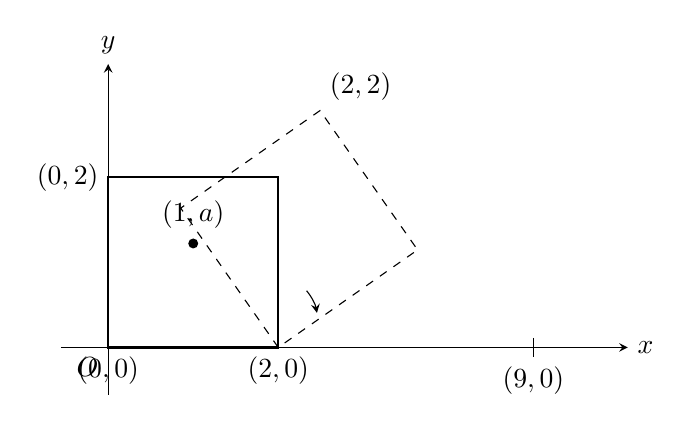
\begin{tikzpicture}[scale=1.2, >=stealth]
    \draw[->] (-0.5,0) -- (5.5,0) node[right] {$x$};
    \draw[->] (0,-0.5) -- (0,3.0) node[above] {$y$};
    \node[below left] at (0,0) {$O$};

    \draw[thick] (0,0) rectangle (1.8, 1.8);
    \node[left] at (0, 1.8) {$(0,2)$};
    \node[below] at (0,0) {$(0,0)$};
    \node[below] at (1.8,0) {$(2,0)$};

    \coordinate (P) at (0.9, 1.1);
    \fill (P) circle (1.5pt);
    \node[above=2pt] at (P) {$(1,a)$};

    \begin{scope}[shift={(1.8,0)}, rotate=35]
      \draw[dashed] (0,0) rectangle (1.8, 1.8);
      \node[above right] at (1.8, 1.8) {$(2,2)$};
    \end{scope}

    \draw[->] (2.1, 0.6) arc (40:10:0.5);

    \draw (4.5, 0.1) -- (4.5, -0.1) node[below] {$(9,0)$};
  \end{tikzpicture}
\end{figure}

\end{document}
